
\documentclass[article]{IEEEtran}
\usepackage{graphicx}
\usepackage{float}
 \usepackage{url}
\usepackage{amsmath}
\setlength{\parskip}{0.5em}
\setlength{\parindent}{2em}

\begin{document}

\title{Fundamentals of Artificial Intelligence Assignment 2- Solving the Travelling Salesman Problem with Genetic Algorithms}

\author{\IEEEauthorblockN{Craig Heptinstall}
\IEEEauthorblockA{Crh13- 110005643\\SEM6120\\
Institute of Computer Science\\
Aberystywth University}}

\maketitle

\begin{abstract}
Genetic algorithms provide an optimization technique for a wide variety of problems, including that of the travelling salesman. The number of solutions for a TSP can become exponential, which genetic algorithms such as roulette, tournament and others can help reduce the number of evaluated solutions vastly. 
\end{abstract}

\section{Introduction}
Genetic algorithms are considered in a wide array of problems where exact algorithms would struggle. The travelling salesman problem is a great example of a problem that does not have a means of finding the best solution first time, and would be increasingly time consuming to loop through all possible solutions to find the lowest cost (length of path).

\subsection{Travelling Salesman Problem}
To understand the travelling salesman problem, the reasons for its existence and early sources should be known. The travelling salesman problem was thought up in 1930 \cite{1} by Merrill Flood whilst looking to solve a school bus routing problem. The problem stems off from the Hamiltonian cycle puzzle, requiring the solver to visit all node or ‘cities’ once in a set of \( \mathcal{N} \) cities. At this point in time, no general method of solution is known \cite{2} (so is considered NP-hard) therefore only the best and shortest paths can be evaluated from several attempts. \par
Because of the nature of the problem, genetic algorithms appear as an idealistic means of finding optimised tours where a solution cannot be found using a mathematical means. Evolutionary algorithms used in genetics may never be guaranteed to find optimal solutions, though due to their random nature they will often find a good solution \cite{3}. Genetic algorithms are called as so because of the similar way they act to natural selection, with the best and most efficient parents creating more advantageous children. In the instance of the travelling salesman, this could be reflected where two parents whose path distances are short are combined to form a child who uses similar paths to that of its parents, combined with a small form of randomness in the hope of improving upon a solution. \par
Figures \ref{fig:1} and \ref{fig:2} show an example TSP with a low number of points where an optimal solution can be found quite easily by exact, heuristic or GA means. An important aspect expressed in figure 2 is that although all the points are visited, the final vertex visited must also be linked to the first in order to return to the starting position.
\begin{figure}
\centering
  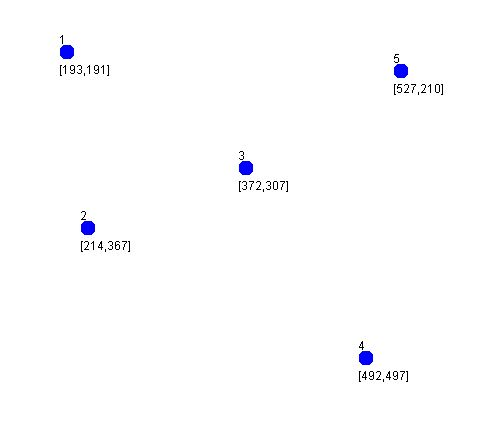
\includegraphics[width=.8\linewidth]{images/problem}
  \caption{An example set of vertices where a travelling salesman problem is present.}
  \label{fig:1}
\end{figure}
\begin{figure}
\centering
  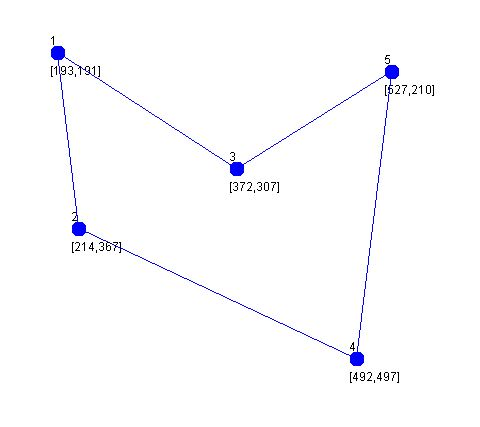
\includegraphics[width=.8\linewidth]{images/solution}
  \caption{A possible solution to the TSP expressed above.}
  \label{fig:2}
\end{figure}

\section{Genetic algorithms considered for TSP}
Before looking at the possible genetic algorithms to be considered for such a puzzle as the TSP, it should be understood that a very basic generic algorithm can be used for such a purpose. In a paper in the Scientific World Journal \cite{4}, a team worked on using a traditional algorithm created back in 1989 by David Goldberg \cite{5} and improving its efficiency to help solve the TSP quickly and as accurately as possible. The original genetic algorithm, which many algorithms are based from today goes through the following process:
\begin{enumerate}
\item Randomly generate an initial population of chromosomes.
\item Use the fitness function to select the fitter chromosomes.
\item Apply the crossover and mutation operators in order. 
\item If a stopping criterion is satisfied, then stop and output the best chromosome
\item Go back to step 2
\end{enumerate}

\section{Proposed solution}
The following sub sections of this paper discusses the merits and drawbacks of using certain genetic algorithm selection strategies. Testing the capabilities of GA's using different means of selecting individual chromosomes (or tour solutions in the case of the travelling salesman problem) will allow statics and conclusions to be applied to the respective strategies, and have a higher chance of finding best possible results for the TSP problem. Alongside selection, the concept of elitism is looked at. Elitism may prevent strong solutions being lost on mutation and crossover, and therefore create better, faster-found routes. 

\subsection{Considered and selected GA representations}
As already discussed in the previous section of the paper, most GA's have been based off of older ones such as chromosome representation \cite{5}. For the purpose of this paper, the algorithm used for the TSP will be also based on this algorithm though different aspects such as crossover, mutation and elitism types will be looked at. To keep the algorithm at a simple chromosome state will allow easier implementation of the algorithm in code form, therefore will be easier to manipulate and change specific aspects to allow for statistical research. \par
There are three parts of the genetic algorithm that will be heavily considered in this paper, each of which will be modified and replaced by other means to compare and find the most optimal solutions to the travelling salesman problem. The three which are integral to any good GA, and which will be explained the need for in the TSP in the following sections are:
\begin{enumerate}
\item Selection- Selects two 'parents' from the current population, usually picking two strong chromosomes is ideal in order to ensure a strong 'child' is created. This like nature, as the strongest usually survive and again produce offspring which inturn makes the population stronger as a whole.
\item Crossover- The algorithm responsible for mating the two parents selected in the previous state of the GA. By mixing the two parents as efficiently as posisble, two strong child chromosomes should be created using traits from both parents. 
\item Mutation- Once the population has been updated with its new chromosomes formed from previous solutions, there should be some small amount of mutation to some of the the chromosomes. This allows the random chance that the solution could get better in some cases, therfore when selected and mated again the overall population may get better.
\end{enumerate}
Each of these components of the GA to be used in the application will be descirbed in the following section, each of which provided alongside how the application could implement them.

\subsubsection{Selection methods}
In order to create the most efficient child chromosomes (or path around TSP nodes in this case), there a range of availible algorithms that can be used to select parent chromosomes. There are subcategories of selection stratedgies which are explained in some depth on Marek Obitko's 'Introduction to genetic algorithms' \cite{6} . The first of which should be explored is the simple but effective roulette wheel selection technique. This works by imagining all the solututions are placed as roulette wheel numbers, with each solution having a proportion of the wheel decided by its fitness value. \par
A radnomly genertaed number between zero and the total fitness of the population is then selected, and starting with the chromosomes with the higher fitness values, there fitness is subtracted from the random number until that number equals or is below zero. This process stops and the that chromosome is returned as a parent. This could be compared to the roullette ball stopping on a track. \par
By having the roulette wheel broken up by the size of fitness values, the larger the fitness value means the better chance of being selected. When a random number is selected, Figure \ref{fig:3} shows how some chromosomes could be placed onto a roulette wheel system. 
\begin{figure}[H]
\centering
  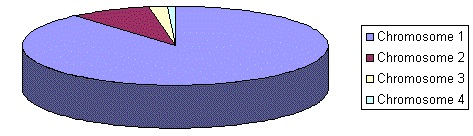
\includegraphics[width=.8\linewidth]{images/rouletteWheel}
  \caption{A roulette wheel example showing a single chromosome with a far better fitness than the others.}
  \label{fig:3}
\end{figure}
To implement this into a TSP solver application, this will be done by simply looping through all of the paths, getting a total fitness and then looping again deducing each fitness value until zero is reached. This will be the simplest of the algorithms to implement and should be made to be built upon for other such algorithms like rank based ones. \par
The issue with roulette selection which is solved by the second selection method whcih will be used by a proposed TSP solver applicaation is that if there is a clear best chromosome with a fitness value that differs largly from the others then its chance of getting selected to be a parent may be two high, therefore childs formed may always be from parents which are the same. This defeats the purpose of the crossover. \par
To solve this, a function called rank selection was created to keep in mind that although chromosomes with better fitness should have a higher chance of being selected, but they should have more of an exponential system to keep chances fair. Therefore, rank based system simply assigns the best fiteness chromosome with a higher standard number, and this number is decreased as the rank of each chromosome is less. For example, with a population of 5, the best chromosome would be assigned the rank 5, and the next 4 and so on. This then means that although the roulette ball will still have the possibibilty of landing on any chromosome, the chances of landing on higher and lower fiteness chromosomes wil be biased more fairly. Figure \ref{fig:4} shows an example rank system in use with a set of chromosomes.
\begin{figure}[H]
\centering
  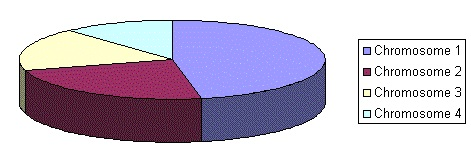
\includegraphics[width=.8\linewidth]{images/rank}
  \caption{An improved form of the roulette wheel with a fairer system of laying out chromosomes.}
  \label{fig:4}
\end{figure}
In the case of this TSP solver application, this could be done by firstly comparing each of the path lengths in the population, and then ordering them by lowest fitness first. Once this is complete, a fitness can be assigned to each starting with the population size, and decreasing the value of the fitness by one with each iteration. Once they are ranked, the roulette wheel method can use the edited population.\par
The third and final selection technique to be explored that will be tested in a TSP solver application will be tournament selection method. This uses a different mechanism to the previous two, by only evaluating a given number of solutions in a population rather than the entire population. Using the defined number of randomly selected chromosomes, the algorithm then gets the fitness of each and returns the winning chromosome. The tournament selection method ensures that weaker chromosomes do not make it through to the next evolution. In the case of the proposed application, this would be a simple implementation of a method which takes a population, a requested tournament size, and then uses a random number generator to select solutions before competing them together to return a winner. 

\subsubsection{Crossover methods}
The next integral part of the genetic algorithm to be implemented is the crossover type. For this, two methods have been considered; ordered and uniform. Alike the previous section, both will be discussed how they function and how they will be integrated within the solver application. \par
The reason for only selecting two crossover methods stems from the reason that although many crossover algorithms exist, many of them are inconsistant a probelm such as travelling salesman. For instance, take the crossover example in figure \ref{fig:5}, after a simple one-point crossover, although the chromosomes have been mixed, the solutions in the childs are no longer valid since not all the points will be visited. A paper by Kylie Bryant which looks at both general genetic algorithms and how they can be applied to the travelling salesman problem mentions that algorithms should be made to make sure that children chromosomes do not finish as illeagle solutions, and that 'in this way, crossover is very problem specific' \cite{7}. \par
The first to be considered is ordered crossover. The same paper explains this type of crossover well, explaining that this type of crossover is very similar to the PMX (partially mapped crossover) method, except instead of repairing chromesomes which contain repeat nodes, the rest of the nodes are rearranged to provide a leagal path.
PAGE 14 INFEASABLE CROSSOVERS
The second crossover algorithm 

\subsubsection{Mutation methods}

\subsubsection{Evolution stop criteria}

\subsection{Application structure}
Folllowing the completion of research into various implementation options for different parts of the TSP solver application, the structure of the application itself can be detailed. In order to do this, a high level class diagram, alongside a description of communication between classes has been provided in Figure \ref{6}. The language chosen for this implimentation was Java, for its extensive library collections and vast amount of tutorials similaly using the language for other genetic algorithm examples.
\begin{figure}[H]
\centering
  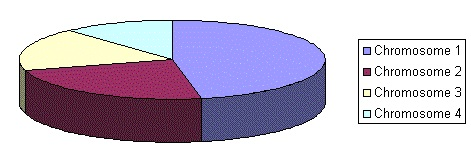
\includegraphics[width=.8\linewidth]{images/rank}
  \caption{High level class diagram of the TSP solver application.}
  \label{fig:6}
\end{figure}
As it can be seen in the diagram, there is a GUI in the design which is seperated from the main logic of the application. This was done in order S

\subsection{Comparison of application results}

\section{Overall findings and conclusion}

\subsection{Improvements to proposed solution}

\begin{thebibliography}{9}

\bibitem{1} 
E.L. Lawler, \textit{The Traveling salesman problem : a guided tour of combinatorial optimization},
1985

\bibitem{2} 
E.W. Weisstein, \textit{Hamiltonian Cycle},
\textit{\url{http://mathworld.wolfram.com/HamiltonianCycle.html}}, 2015

\bibitem{3} 
D.W. Dyer, \textit{When are Evolutionary Algorithms Useful?},
\textit{\url{http://watchmaker.uncommons.org/manual/ch01s02.html}}, 2008

\bibitem{4} 
C.W. Tsai, S.P Tseng, M.C. Chiang, C.S. Yang, T.P. Hong, \textit{A High-Performance Genetic Algorithm: Using Traveling Salesman Problem as a Case},
The Scientific World Journal Volume 2014, 2014

\bibitem{5}
D.E. Goldberg, \textit{Genetic Algorithms in Search, Optimization, and Machine Learning},
Addison-Wesley Longman Publishing Co., 1989. 

\bibitem{6}
M. Obitko, \textit{Introduction to Genetic Algorithms, Selection},
University of Applied Sciences. Czech Technical University., 1998. 

\bibitem{7}
K. Bryant , \textit{Genetic Algorithms and the Traveling Salesman Problem},
Department of Mathematics. Harvey Mudd college., 2000. 

\end{thebibliography}
\end{document}


